\section{Flows around the blocked components}\label{sec:flows}

Fix one time slice $t$.  The graph $\mathcal H_t$ consists of the available slots, including
all $\ell$ slots at every site outside $\Lambda$, with all available slot
pairs across each nearest-neighbor site edge.  Write $\mathcal Z=\mathcal O_t$
for its finite blocked set.  We will represent masses near regular anchors as divergences
of flows with controlled energy.  This will bound their pairing with a
function by that function's Dirichlet energy, the estimate needed for the
cross term in Section~\ref{sec:leakage}.
The divergence and energy viewpoint is the classical electrical-network
flow method; see \cite[Sections~1.3.5 and~2.4.6]{DoyleSnell1984}.
The geometric work here is to retain a quantitative decay bound after
routing through this dependent obstacle configuration.

Give every unoriented slot edge $e$ a reference orientation $(e^-,e^+)$.
A flow is a real function $J$ on these reference edges; its divergence is
outgoing minus incoming flow.  Thus a signed unit path from $a$ to $b$
has divergence $\1_{\{a\}}-\1_{\{b\}}$.  Write
$\dist(e,y)=\min\{|x-y|_\infty:x\text{ is an endpoint site of }e\}$.
Constants in this Section depend only on $d,\ell$ and the fixed geometric
constants in Section~\ref{sec:sparse}, never on the slice or volume.

The construction begins with a full-lattice unit flow whose strength at
distance $h$ from its source is $O((1+h)^{1-d})$.  We replace each oriented
lattice edge by a path through available slots, with endpoints given by
one application of a map on the original vertices.  A short additional
path then restores the source at the specified slot.  The geometry below
bounds the displacement of the replacement paths, and hence the number
of original edges that can contribute to a given available edge.
The resulting decay will let us add flows from a sparse collection of
sources with controlled total energy.

\subsection{Filled hulls and their surviving boundaries}

We first thicken each blocked component to obtain clearance for routes
around it.  After filling the finite pockets of its complement, we will
show that the exterior vertex boundary is connected by sup-norm steps of
length at most one.  These steps can be replaced by unblocked
nearest-neighbor paths.  The filled sets may be nested; their
inclusion-maximal members will give disjoint regions on which to define
the vertex map.

Let $C$ range over the components of $\mathcal Z$ for steps of sup norm
at most eight.  Set
\[
 A_C=\{z\in\Z^d:\dist(z,C)\le4\},\qquad
 H_C=\Z^d\setminus U_C,
\]
where $U_C$ is the infinite nearest-neighbor component of
$\Z^d\setminus A_C$.  Such an infinite component is unique: the exterior
of a box containing $A_C$ is connected when $d\ge2$.  Thus $H_C$ is
$A_C$ with its finite complementary components filled in.  The exterior
vertex boundary of $H_C$ is
\[
 S_C=\{v\notin H_C:\text{some }u\in H_C\text{ satisfies }|u-v|_1=1\}.
\]

The exterior-boundary connectivity in the next lemma is the lattice case
of Tim\'ar's boundary-connectivity result~\cite[Lemmas~1--2]{Timar2013}.
We include the plaquette proof together with the separate hull and
clearance estimates needed for the routes.

\begin{lemma}[Hull topology and clearance]\label{lem:hulls}
Let $d\ge2$ and let $\mathcal Z\subset\Z^d$ be finite.  The sets $A_C$
are pairwise disjoint and nearest-neighbor connected.  Each $H_C$ is finite,
is nearest-neighbor connected, has connected complement, and is contained
in the coordinate bounding box of $A_C$.  Any two hulls are disjoint or one
contains the other.

For every edge $\{u,v\}$ with $u\in H_C$, $v\notin H_C$,
\begin{equation}\label{eq:hull-clearance}
 \dist(u,C)=4,\qquad \dist(v,C)=5.
\end{equation}
Both endpoints are unblocked.  The set $S_C$ is connected by steps of sup
norm at most one.  Each such step can be replaced by a nearest-neighbor
path of unblocked sites, contained in the unit enlargement of the bounding
box of $A_C$.  Consequently any two points of $S_C$ can be joined by a
finite path of unblocked sites in that enlargement.
\end{lemma}

\begin{proof}
Distinct components have mutual distance at least nine, so their
radius-four thickenings are disjoint.  The radius-four lattice cubes about
successive points of a component intersect; their union is connected.
Every finite complementary component has a neighbor in $A_C$, which proves
that filling preserves connectivity.  A vertex outside the coordinate
bounding box has a coordinate ray avoiding that box, so it belongs to
$U_C$.  This proves finiteness and the claimed containment.

For laminarity, take two disjoint connected thickenings $A_C,A_{C'}$.
The second lies in a single component of the complement of the first.
If it lies in a finite component, then $U_C$ is an infinite connected
subset of the complement of $A_{C'}$, whence $U_C\subset U_{C'}$ and
$H_{C'}\subset H_C$.  The reversed containment is treated identically.
In the remaining case each thickening lies in the infinite complementary
component of the other.  Then $H_C$ avoids $A_{C'}$ and is connected;
since it contains $A_C\subset U_{C'}$, it lies wholly in $U_{C'}$.
Hence $H_C$ and $H_{C'}$ are disjoint.

We next prove connectivity of the exterior boundary without a planar
separation argument.  Let $\mathcal E_C$ be the edges between $H_C$ and
$U_C$, and join two of these edges when they lie on an elementary lattice
plaquette.  Every plaquette meets $\mathcal E_C$ an even number of times,
and all cut edges of one plaquette belong to the same component of this
edge relation.  Thus each component separately meets every plaquette
evenly.  It then meets every finite closed lattice walk evenly: modulo two,
such a walk is a sum of elementary plaquettes, as follows by commuting
successive steps in different coordinate directions and canceling inverse
steps.  If the cut had two components, take one edge from each, join their
inner endpoints within $H_C$ and their outer endpoints within $U_C$.
The resulting closed walk uses exactly one cut edge from each chosen
component, a contradiction.  The cut is therefore connected by plaquettes.
The outer endpoints of cut edges on a common plaquette have sup distance
at most one.  This proves the asserted connectivity of $S_C$.

An inner cut endpoint $u$ must belong to $A_C$: otherwise a complementary
pocket containing $u$ would be adjacent to the infinite component through
$v$, which is impossible.  Since $v\notin A_C$ and $|u-v|_\infty=1$,
the distances to $C$ are exactly four and five.  For another component
$C'$, separation gives $\dist(v,C')\ge4$ and $\dist(u,C')\ge5$.
To interpolate a sup step between two points of $S_C$, change the differing
coordinates one at a time.  Every intermediate vertex is within sup
distance one of its starting point, hence has distance at least four
from $C$ and at least three from every other component.  All these
vertices survive.  They also remain in the coordinate bounding box of
$S_C$, which is contained in the unit enlargement stated above.
\end{proof}

Keep only the inclusion-maximal hulls and denote their family by
$\mathfrak H$.  They are pairwise disjoint and contain all blocked sites.
Choose one representative $r_H\in S_C$ for each $H=H_C\in\mathfrak H$,
and define a map on sites by
\begin{equation}\label{eq:once-only-map}
 \rho(z)=
 \begin{cases}
 r_H,&z\in H\in\mathfrak H,\\
 z,&z\notin\bigcup_{H\in\mathfrak H}H.
 \end{cases}
\end{equation}
All images are unblocked.  The map is applied once.  A representative
can lie in another hull, so no identity $\rho(r_H)=r_H$ is assumed.

For each oriented lattice edge $(u,v)$, join $\rho(u)$ to $\rho(v)$ as
follows.  If both endpoints are in the same hull, use the empty path.
If neither is in a hull, use the edge itself.  If only $u$ belongs to a
hull $H$, then $v\in S_C$ and a path along its surviving boundary joins
$r_H$ to $v$; reverse this prescription when only $v$ is in a hull.
Finally, if $u\in H$ and $v\in H'$ for distinct maximal hulls, both
$u$ and $v$ survive and the signed route is
\begin{equation}\label{eq:adjacent-hull-route}
 r_H\ \longrightarrow\ v\ \longrightarrow\ u\ \longrightarrow\ r_{H'}.
\end{equation}
The first portion uses the exterior boundary of $H$, the last the exterior
boundary of $H'$, and the middle portion traverses the original edge in
reverse.  Indeed $v\in S_C$ and $u\in S_{C'}$.  Erase loops from the
resulting walk, leaving a simple path with the same endpoints.  This path
stays in the enlarged bounding boxes of the hulls incident to the original
edge, together with that edge.  Figure~\ref{fig:hull-routing} shows an
exterior-boundary detour and the adjacent-hull case in which the one-use
convention and the sign of the middle portion matter.

\begin{figure}[tbp]
\centering
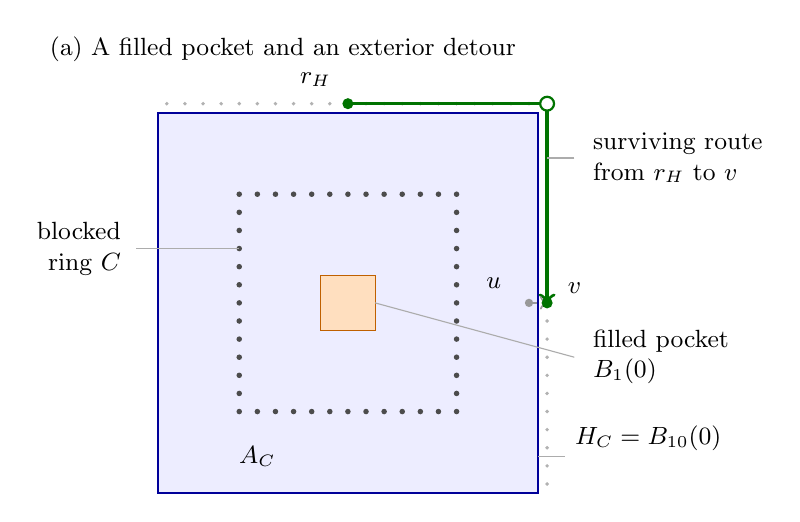
\begin{tikzpicture}[x=.23cm,y=.23cm,font=\small]
  \node[anchor=west] at (-17,14)
    {(a) A filled pocket and an exterior detour};
  \fill[blue!7] (-10.5,-10.5) rectangle (10.5,10.5);
  \draw[blue!60!black,thick] (-10.5,-10.5) rectangle (10.5,10.5);
  \fill[orange!25] (-1.5,-1.5) rectangle (1.5,1.5);
  \draw[orange!75!black] (-1.5,-1.5) rectangle (1.5,1.5);
  \foreach \n in {-6,...,6} {
    \fill[black!70] (\n,6) circle (1pt);
    \fill[black!70] (\n,-6) circle (1pt);
  }
  \foreach \n in {-5,...,5} {
    \fill[black!70] (6,\n) circle (1pt);
    \fill[black!70] (-6,\n) circle (1pt);
  }
  \foreach \n in {-10,...,10} {
    \fill[gray!60] (\n,11) circle (.7pt);
    \fill[gray!60] (11,\n) circle (.7pt);
  }
  \draw[->,green!45!black,very thick] (0,11)--(11,11)--(11,0);
  \draw[->,gray!80,dashed,thick] (10,0)--(11,0);
  \fill[green!45!black] (0,11) circle (2pt);
  \fill[green!45!black] (11,0) circle (2pt);
  \fill[gray!80] (10,0) circle (1.5pt);
  \filldraw[fill=white,draw=green!45!black,thick] (11,11) circle (2.5pt);
  \node[anchor=south east] at (-.4,11.4) {$r_H$};
  \node[anchor=east] at (9,1.1) {$u$};
  \node[anchor=west] at (11.6,.8) {$v$};
  \node at (-5,-8.5) {$A_C$};
  \node[anchor=west] at (12,-7.5) {$H_C=B_{10}(0)$};
  \draw[gray!65] (12,-8.5)--(10.5,-8.5);
  \node[anchor=east,align=right] at (-12,3)
    {blocked\\ring $C$};
  \draw[gray!65] (-11.7,3)--(-6,3);
  \node[anchor=west,align=left] at (13,-3)
    {filled pocket\\$B_1(0)$};
  \draw[gray!65] (12.5,-3)--(1.5,0);
  \node[anchor=west,align=left] at (13,8)
    {surviving route\\from $r_H$ to $v$};
  \draw[gray!65] (12.5,8)--(11,8);
\end{tikzpicture}
\par\medskip
\begin{tikzpicture}[x=.55cm,y=.4cm,font=\small]
  \node[anchor=west] at (-4,5.5)
    {(b) Adjacent hulls exchange representatives};
  \fill[blue!7] (-4,-4) rectangle (4,4);
  \draw[blue!60!black,thick] (-4,-4) rectangle (4,4);
  \fill[orange!10] (5,-4) rectangle (13,4);
  \draw[orange!75!black,thick] (5,-4) rectangle (13,4);
  \draw[gray!55] (-4.5,0)--(13.5,0);
  \foreach \x in {-4,...,13} {\fill[gray!60] (\x,0) circle (1pt);}
  \fill (0,0) circle (2.5pt);
  \fill (9,0) circle (2.5pt);
  \node[above=5pt] at (0,0) {$0$};
  \node[above=5pt] at (9,0) {$9e_1$};
  \node at (0,3.1) {$H_0=[-4,4]^d$};
  \node at (9,3.1) {$H_1=9e_1+[-4,4]^d$};
  \draw[fill=white,blue!65!black,thick] (5,0) circle (3pt);
  \draw[fill=white,orange!80!black,thick] (4,0) circle (3pt);
  \node[anchor=north east] at (3.8,-.5) {$u=4e_1=r_{H_1}$};
  \node[anchor=north west] at (5.2,-.5) {$v=5e_1=r_{H_0}$};
  \draw[->,gray!80,dashed,thick] (4,1)--(5,1);
  \node[above=3pt,fill=white,inner sep=1.5pt] at (4.5,1) {original edge};
  \draw[->,blue!65!black,very thick] (5,-2.3)--(4,-2.3);
  \node[below=4pt,fill=white,inner sep=1.5pt] at (4.5,-2.3) {routed edge};
  \node[align=center] at (4.5,-5.3)
    {$\rho(u)=v,\quad\rho(v)=u$
     \\ $\operatorname{div}\1_{v\to u}=\1_{\{v\}}-\1_{\{u\}}$};
\end{tikzpicture}
\caption{Replacing lattice edges by surviving paths.
In (a), a two-dimensional example, $C=\{z:|z|_\infty=6\}$ is a blocked
ring.  Its radius-four thickening is
$A_C=\{z:2\le|z|_\infty\le10\}$; filling the surviving pocket
$B_1(0)$ gives $H_C=B_{10}(0)$.  The original edge $u\to v$, with
$u=(10,0)$ and $v=(11,0)$, is replaced by the indicated path from
$r_H=(0,11)$ to $v$.  The open corner is a surviving interpolation
vertex outside $S_C$: a nearest-neighbor route need not remain in $S_C$
itself.  In (b), the only blocked sites are $0$ and $9e_1$.
Their filled radius-four hulls are the two
displayed lattice cubes, shown schematically in a coordinate slice; the
transverse scale is compressed.  Both $u=4e_1$ and $v=5e_1$ survive.
Choosing $r_{H_0}=v$ and $r_{H_1}=u$ sends the oriented original edge
$u\to v$ to the reverse edge $v\to u$.  This is the case of
\eqref{eq:adjacent-hull-route} in which the two boundary portions are
empty.  Applying $\rho$ again would undo this required image exchange.
Panel (a) illustrates the definitions in $d=2$; the hull and boundary
properties in every $d\ge2$ are proved in Lemma~\ref{lem:hulls}.}
\label{fig:hull-routing}
\end{figure}

\FloatBarrier

\subsection{A decaying unit flow from every nearby slot}

The topology gives routes for all lattice edges.  Regularity now bounds
their displacement, which will bound the number of routes using any one
target edge.

\begin{proposition}[Decay of a routed unit flow]\label{prop:flow-decay}
Let $d\ge3$, $\nu=1/(100d)$, and suppose the anchor $x$ is regular in the
sense of Definition~\ref{def:regular-anchor}.  Fix the local constant
$M_*$ as in~\eqref{eq:local-radius-choice} and take $R$ sufficiently
large in terms of those fixed constants.  For every available slot $a$
at any site $y\in B_R(x)$ there is a flow $J_a$ on the available-slot
graph such that
\begin{equation}\label{eq:flow-envelope}
 \operatorname{div}J_a=\1_{\{a\}},\qquad
 |J_a(e)|\le C(1+\dist(e,y))^{-k},
 \qquad k=d-1-d\nu.
\end{equation}
In particular, $\sum_e J_a(e)^2<\infty$.
\end{proposition}

\begin{proof}
First we quantify the hull sizes.  A blocked component meeting $B_{10R}(x)$
has fewer than $2d$ vertices.  Otherwise, starting at a vertex there,
a connected exploration would find $2d$ vertices within $2d-1$ component
steps, all in a ball of radius $8(2d-1)\le M_*$, contradicting regularity.
Such a component has diameter at most $8(2d-2)$, and its hull has diameter
at most
\[
 D_{\mathrm{loc}}=8(2d-2)+8.
\]
For a component avoiding $B_{10R}(x)$, let
$b_C=\min_{z\in C}|z-x|_\infty>10R$.  Applying remote regularity at a
minimizer gives
\begin{equation}\label{eq:remote-hull-size}
 \operatorname{diam}H_C\le 2(1+b_C)^\nu+8.
\end{equation}
This also bounds the diameter of its coordinate bounding box.  Since
$\nu<1$, increasing a fixed lower threshold for $R$ makes the right side,
plus any of the fixed enlargements used above, at most $b_C/10$.
All sites of these enlarged boxes then have distance comparable to $b_C$
from every $y\in B_R(x)$.  In particular, no such remote box contains $y$.

Apply the routes following~\eqref{eq:once-only-map}, using fixed choices
of representatives and paths.  The preceding size bounds show that the
route of a lattice edge $e$ lies within distance
\begin{equation}\label{eq:routing-displacement}
 C(1+\dist(e,y))^\nu
\end{equation}
of that edge.  For a local hull this is the fixed bound $D_{\mathrm{loc}}+2$.
For each remote hull incident to $e$, an endpoint of $e$ belongs to its
bounding box, so its $b_C$ is comparable to $1+\dist(e,y)$; now use
\eqref{eq:remote-hull-size}.  The same reasoning applies when the edge
joins two hulls.  These comparisons are uniform over all injection sites
$y\in B_R(x)$.

Choose one canonical available slot $c(z)$ at each unblocked site $z$.
Lift every routed site path to these canonical slots.  All its edges exist
because every pair of available slots across a lattice edge is present.
The map of the original lattice vertices into slots is
$\psi(z)=c(\rho(z))$.  Its preimages are finite: outside the finitely many
finite hulls it is injective, and only those hulls can supply additional
preimages.

We also need a bounded path from the specified slot $a$ to $\psi(y)$.
If $y$ is in a hull, that hull is local and the separation between $y$
and $\rho(y)$ is at most $D_{\mathrm{loc}}+1$.  Both sites are unblocked, so
Lemma~\ref{lem:local-connectivity} joins them through survivors in a
fixed neighborhood of $y$.  Its assumptions hold because $y\in B_R(x)$,
the neighborhood has fixed radius, and $R$ dominates that radius.
Lift this path, starting at $a$.  If $\rho(y)=y$ but $a\ne c(y)$,
use a two-edge path through a surviving neighbor of $y$.  Such a neighbor
exists, since blocking all $2d$ neighbors would violate local regularity.
Thus in all cases there is a simple slot path $Q_a$ from $a$ to $\psi(y)$
of bounded length and displacement.  The choice
$K_{\rm conn}\ge8(2d-2)+12$ in the local-connectivity construction covers
these requirements before $M_*$, $R$, and finally $p$ are fixed.

Start with an explicit unit flow $F_y$ on the full lattice.  In the
positive orthant based at $y$, give each site $y+n$, $n\in\Z_{\ge0}^d$,
$|n|_1=N$, mass
\[
 a_N=\binom{N+d-1}{d-1}^{-1},
\]
and send the fraction $(n_j+1)/(N+d)$ along its edge in direction $e_j$.
Put zero on all other edges.  At a site $y+n$ of level $N\ge1$, the
incoming mass is
\[
 a_{N-1}\frac{\sum_j n_j}{N+d-1}
 =a_{N-1}\frac{N}{N+d-1}=a_N,
\]
which equals its outgoing mass.  The outgoing mass at $y$ is one.
Consequently
\begin{equation}\label{eq:orthant-flow}
 \operatorname{div}F_y=\1_{\{y\}},\qquad
 |F_y(e)|\le C(1+\dist(e,y))^{1-d}.
\end{equation}

For each lattice edge, send its signed $F_y$-value along its lifted simple
path.  To justify this infinite sum and estimate it, fix a target slot
edge $f$ and write $h=\dist(f,y)$.  If the route of an original edge $e$
uses $f$, put $t=\dist(e,y)$.  The displacement bound gives
\[
 |h-t|\le C(1+t)^\nu+C.
\]
Because $\nu<1$, this implies $1+t\asymp1+h$, with uniform constants:
above a fixed threshold the error is at most $(1+t)/2$, and below that
threshold all quantities are bounded.  It follows also that $e$ lies
within distance $C(1+h)^\nu$ of $f$.  There are at most
\begin{equation}\label{eq:target-congestion}
 C(1+h)^{d\nu}
\end{equation}
such lattice edges.  Each routed path is simple, so any one of them uses
$f$ at most once.  Summing~\eqref{eq:orthant-flow} over this finite set
gives a well-defined flow $J_a^0$ with
\[
 |J_a^0(f)|\le C(1+h)^{1-d+d\nu}.
\]
The count~\eqref{eq:target-congestion} already counts all contributions
to $f$; no path-length factor is present.

Local finiteness of the path sum and finiteness of the vertex preimages
justify the divergence calculation at any slot $b$:
\begin{align*}
 \operatorname{div}J_a^0(b)
 &=\sum_{e=(u,v)}F_y(e)
       \bigl(\1_{\{\psi(u)=b\}}-\1_{\{\psi(v)=b\}}\bigr)\\
 &=\sum_{z:\psi(z)=b}\operatorname{div}F_y(z)
 =\1_{\{\psi(y)=b\}}.
\end{align*}
Here one fixed orientation is used for each original lattice edge; the
signed route is always from $\psi(u)$ to $\psi(v)$.  Adding the unit path
flow from $a$ to $\psi(y)$ therefore gives
\[
 J_a=J_a^0+\1_{Q_a},\qquad
 \operatorname{div}J_a=\1_{\{a\}}.
\]
The connector has fixed bounded support near $y$, so enlarging $C$
preserves the envelope~\eqref{eq:flow-envelope}.  Finally,
$2k>d$ for $d\ge3$, and the number of slot edges at radius $h$ is at
most $C(1+h)^{d-1}$.  Squaring the envelope and summing proves finite
energy.  Equivalently, this is a unit flow to infinity: its net outward
flux across any finite vertex set containing $a$ is one.
\end{proof}

\subsection{Overlap and arbitrary subunit injections}

We now combine the individual flows.  Their decay, rather than a
disjointness property of their routes, controls their total energy.

\begin{lemma}[Overlap of two flows]\label{lem:flow-overlap}
Suppose two flows on an available-slot graph obey
\[
 |J(e)|\le C_0(1+\dist(e,y))^{-k},\qquad
 |J'(e)|\le C_0(1+\dist(e,y'))^{-k},
\]
where $d/2<k<d$.  Then
\begin{equation}\label{eq:flow-overlap}
 \sum_e |J(e)J'(e)|
 \le C(1+|y-y'|_\infty)^{-(2k-d)},
\end{equation}
where $C$ depends only on $d,\ell,k,C_0$.
\end{lemma}

\begin{proof}
Write $H=1+|y-y'|_\infty$.  For bounded $H$ the assertion follows by
summing the squared envelopes and Cauchy--Schwarz.  Otherwise, in the
ball of radius $(H-1)/3$ about either center, the other envelope is at
most $CH^{-k}$, whereas the sum of the nearer envelope is at most
$CH^{d-k}$.  These two regions cost $CH^{d-2k}$.  In the remaining
region the two distances are comparable.  Dyadic annuli of radii
comparable to $2^jH$, $j\ge0$, cost at most
\[
 C\sum_{j\ge0}(2^jH)^{d-2k}\le CH^{d-2k},
\]
since $2k>d$.  Changing a site distance to the distance from an incident
edge changes it by at most one, and the number of slot edges per site
is bounded by $2d\ell^2$.  Thus the same estimates apply to the stated
edge sum.
\end{proof}

\begin{proposition}[Energy for arbitrary injections]\label{prop:flow-energy}
Let $d\ge3$, $\alpha=1/100$, and $\nu=1/(100d)$.  Fix $M_*$ as in
\eqref{eq:local-radius-choice} and take $R$ sufficiently large as in
Proposition~\ref{prop:flow-decay}.  Let $T$ be a finite
set of $m$ anchor slots with sites $x_i$, satisfying
\[
 \#\{i\in T:x_i\in B_h(z)\}\le L(1+h)^\alpha
 \quad\text{for all }z\in\Z^d,\ h\ge0.
\]
Fix an available-slot graph and a subset $I\subset T$ of anchors regular
for this graph.  For each $i\in I$, let $\mu_i$ be any nonnegative mass
on its slots, supported over $B_R(x_i)$ and satisfying
$\sum_a\mu_i(a)\le1$.  There is a flow $J$ such that
\begin{equation}\label{eq:injection-flow-energy}
 \operatorname{div}J=\sum_{i\in I}\mu_i,
 \qquad \sum_e J(e)^2\le C|I|R^\alpha\le CmR^\alpha.
\end{equation}
Consequently every finitely supported real function $g$ on the graph
satisfies
\begin{equation}\label{eq:injection-pairing}
 \left|\left\langle\sum_{i\in I}\mu_i,g\right\rangle\right|
 \le \bigl(CmR^\alpha\mathcal D(g)\bigr)^{1/2},
 \qquad \mathcal D(g)=\frac12\sum_e(g(e^-)-g(e^+))^2.
\end{equation}
All constants are uniform over the choices of $I$ and of the masses.
\end{proposition}

\begin{proof}
The empty case uses $J=0$.  Otherwise, for each slot $a$ in the support
of $\mu_i$, take a unit flow $J_{i,a}$ from
Proposition~\ref{prop:flow-decay}, using anchor $x_i$, and set
\[
 J=\sum_{i\in I}\sum_a\mu_i(a)J_{i,a}.
\]
This is a finite linear combination, and its divergence is as asserted.
Put $q=2k-d=d-2-2d\nu>\alpha$.  By
Lemma~\ref{lem:flow-overlap}, the absolute overlap of $J_{i,a}$ and
$J_{j,b}$ is at most $C(1+|y_a-y_b|_\infty)^{-q}$, where $y_a,y_b$
are the sites of their injection slots.  If $|x_i-x_j|_\infty>4R$,
then $|y_a-y_b|_\infty\ge |x_i-x_j|_\infty/2$, uniformly over both
supports.  For the remaining anchor pairs use the uniform constant
overlap bound.  The mass bound of one per anchor therefore gives
\[
 \sum_eJ(e)^2\le C\sum_{i\in I}
 \left[\#\{j\in I:|x_j-x_i|_\infty\le4R\}
 +\sum_{\substack{j\in I\\|x_j-x_i|_\infty>4R}}
     (1+|x_j-x_i|_\infty)^{-q}\right].
\]
The first term is at most $CL R^\alpha$.  Splitting the second into
annuli $2^j4R<|x_j-x_i|_\infty\le2^{j+1}4R$ bounds it by
\[
 CL\sum_{j\ge0}(2^jR)^{\alpha-q}\le C,
\]
because $R\ge1$ and $q>\alpha$.  This proves
\eqref{eq:injection-flow-energy}, including repeated anchor sites since
the growth assumption counts slots.

Finally, finite support of $g$ permits summation by divergence without a
term at infinity:
\[
 \left\langle\sum_i\mu_i,g\right\rangle
 =\sum_e J(e)(g(e^-)-g(e^+)).
\]
Cauchy--Schwarz and $\sum_e|\nabla_e g|^2=2\mathcal D(g)$ give
\eqref{eq:injection-pairing}.  In particular it applies to functions that
vanish on the killed boundary and outside the physical box, with exactly
the energy normalization in~\eqref{eq:slot-energy}.
\end{proof}

The construction is deterministic at a single slice.  Thus the masses
and the set of regular anchors may depend on the whole exposed
environment; the pairing bound requires neither independence nor a
choice of flows continuous in time.
